\section{Einleitung}

\subsection{Definition: Smart Home} % TODO redo this section

Wörtlich übersetzt, bedeutet der englische Begriff Smart Home so viel wie \textit{intelligentes Zuhause}. Intelligent meint hierbei die digitale und automatische Steuerung der Haustechnik.

Im Allgemeinen steht Smart Home dafür, für eine intelligente Vernetzung von elektrischen Verbrauchern in privaten Haushalten mit dem Ziel, den Wohnkomfort, die Sicherheit und die Energieeffizienz des Gebäudes zu steigern.\myfootcite[Vgl.][]{definition_smart_home}

Durch die Smart Home Technologie werden einerseits Alltagsvorgänge automatisiert, andererseits können die Geräte-Einstellungen, z.B. von Heizung, Licht und Lautsprechern, per Computer oder Smartphone schnell an die persönlichen Bedürfnisse angepasst werden ob zuhause oder unterwegs.

\begin{figure}[ht] % TODO this picture has nothing to do with smart home. it displays IOT!
	\centering
	\caption{Smart Home Mobiltelefonsteuerung}
	\includegraphics[width=0.8\textwidth]{smart_home_handy}
	\caption*{\footnotesize{Quelle: \mycite{figure_smart_home_handy}}}
	\label{fig:smarthomehandy}
\end{figure}

\subsection{Fragestellungen} % TODO better title

% monetarisierung von smart home produkten
% beispiele zu existierenden systemen

\section{Evaluation}

\subsection{Internet of Things} % TODO better title

Das Internet der Dinge hat direkt zunächst nichts mit Heimautomatisierung zu tun.

% Abgrenzung iot / smart home

\subsection{Systembeschreibung}

Aschendorf beschreibt den Aufbau von Smart Home Systemen als hierarchisches System.
\autoref{fig:automatisierungspygramide} zeigt die drei Ebenen der Automatisierungspyramide nach Aschendorf:
Die \textit{Feldbusebene}, die \textit{Automatisierungsebene} und die \textit{Leitebene}. \myfootcite[Vgl.][59]{aschendorf14}

\begin{figure}[ht]
	\centering
	\caption{Automatisierungspyramide nach Aschendorf}
	\includegraphics[scale=0.8]{Automatisierungspyramide_nach_Aschendorf}
	\caption*{\footnotesize{Quelle: Eigene Darstellung.}}
	\label{fig:automatisierungspygramide}
\end{figure}

\subsubsection{Feldbusebene}

Die Feldbusebene besteht aus sämtlichen eingebauten Systemkomponenten, also Gateways, welche verschiedene Systeme verbinden, Sensoren, welche z.B. Temperatur und Luftfeuchtigkeit überwachen, und Aktoren, wie z.B. Glühbirnen.
In der selben Ebene finden sich auch die Verbindungen der oben genannten Geräte wieder.
So ist die Feldbusebene in sich bereits funktional und direkt nutzbar.
Es kann z.B. der Sensor \textit{Lichtschalter 3} ausgelöst werden, welcher den Aktor \textit{Deckenlampe Wohnzimmer} aktiviert.\myfootcite[Vgl.][66-67]{aschendorf14}

\subsubsection{Automatisierungsebene}

Geräte übergreifende Automatisierungen werden in der Automatisierungsebene implementiert.
Dies wird durch einfache Controller oder programmierbare Mikrocomputer realisiert.
Nach der Änderung von Zuständen, wie z.B. der aktuellen Zeit, die Anwesenheit eines Bewohners oder die Temperatur eines Raumes, passt sich das Smart Home System mit dieser zusätzlichen Ebene nun nach vorgegebenen Regeln autonom an.\myfootcite[Vgl.][67-68]{aschendorf14}

\subsubsection{Leitebene}

Die Leitebene widmet sich der Interaktion des Smart Home Systems mit dessen Bewohnern.
Es lässt sich die Interaktion teilen in Eingaben und Ausgaben.
Zu den Eingaben zählen Befehle, die z.B. über Steuerungs-Apps gesendet werden oder von einem zentralen Steuerungscomputer emittiert werden.
Ausgaben werden etwa über digitale Dashboards auf diversen Displays angezeigt.
Über dieselben werden meist auch Fehlerdiagnosemeldungen angezeigt.\myfootcite[Vgl.][68-70]{aschendorf14}

% system beschreiben: aus welchen komponenten besteht ein smart home (automation, iot, ...)
% here we can use one of the required methods! (e.g. SSA)

\subsection{Verbindungstypen} % (auswahl)

\subsubsection{LAN und WLAN}
\subsubsection{ZigBee}
\subsubsection{Z-Wave}

\subsection{Amazon Alexa}

% easy to use
% internet required
% data compromised
% closed source

\subsubsection{Vorteile}
\subsubsection{Nachteile}

\subsection{Home Assistant}

Home Assistant ist eine Open-Source-Software für Heimautomatisierung.
Durch den modularen Aufbau der Software können Entwickler einfach neue Smart Home Produkte implementieren.
So sind aktuell 1187 Smart Home Produkte über 46 Kategorien mit Home Assistant nutzbar.\myfootcite[Vgl.][]{hass_components}

\begin{figure}[ht]
	\centering
	\caption{Home Assistant Core Architektur}
	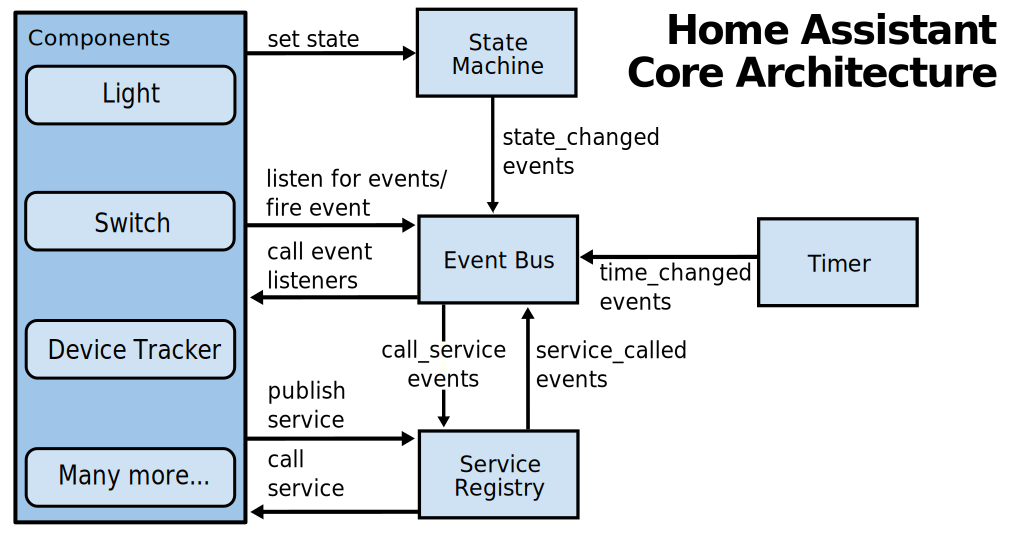
\includegraphics[width=0.9\textwidth]{hass_architecture}
	\caption*{\footnotesize{Quelle: \mycite{hass_architecture_figure}}}
	\label{fig:hasscorearch}
\end{figure}

\autoref{fig:hasscorearch} zeigt die Architektur, welche Home Assistant die Modularität verleiht.
Smart Home Produkte werden als Komponenten implementiert, welche mit dem Home Assistant Core interagieren.
Der Home Assistant Core besteht aus vier Modulen:

Das \textit{State Machine} Modul bildet den Status der verschiedenen Komponenten ab.
Bemerkt ein Fenstersensor z.B. dass ein Fenster geöffnet wurde, aktualisiert die Komponente \textit{Fenstersensor} ihren Status im \textit{State Machine} Modul, indem sie eine Nachricht an das Modul schickt.

Für zeitbasierende Automatisierungen existiert das Modul \textit{Timer}, welches sekündlich ein Event emittiert.
Ein Event ist eine Nachricht, welche beim Auftreten von definierten Bedingungen automatsich verschickt wird.

Über das \textit{Event Bus} Modul werden Events von den beiden bereits genannten Modulen empfangen von diesen ausgehend wiederum Events ausgelöst.

Das \textit{Service Registry} Modul bietet Komponenten die Möglichkeit beim Gesamtsystem einen Service zu registrieren.
Das Gesamtsystem wiederum kann über das selbe Modul den Service einer Komponente in Anspruch nehmen.
So kann eine Glühbirne z.B. den Service \textit{Glühbirne anschalten} registrieren, welcher dann von einer anderen Komponente, z.B. einem Lichtschalter, indirekt, über ein Event, aufgerufen werden kann.

Mit dieser Architektur kann eine neue Komponente implementiert werden, ohne dass der Home Assistant Core berührt wird.
Eine neue Komponente muss lediglich einen Service registrieren, auf ein Event reagieren oder ein Event auslösen können.\myfootcite[Vgl.][]{hass_architecture}
Die Implementierung einer neuen Komponente ist ausführlich in der Home Assistant Dokumentation beschrieben.\myfootcite[Vgl.][]{hass_implement_component}

Veröffentlicht wird Home Assistant unter der Apache 2.0 Lizenz.\myfootcite[Vgl.][]{hass_license}
Die Software ist also kommerziell und privat kostenlos nutzbar.
Lediglich die Marke \textit{Home Assistant} wird geschützt, sowie die Haftung und die Garantie ausgeschlossen.

% Add something about the vision of hass

\myfootcite[Vgl.][]{hass_vision}

\subsubsection{Vorteile}

% great compatibility with A LOT iot products
% open source
% internet not required
% data is stored local

\begin{wrapfigure}{r}{0.4\textwidth}
	\centering
	\caption{ESP8266 Board}
	\includegraphics[scale=.1]{esp8266}
	\caption*{\footnotesize{Quelle: \mycite{esp8266}}}
	\label{fig:esp8266}
\end{wrapfigure}

\subsubsection{Nachteile}

% not easy to use

\subsection{Integerierte Lösungen} % so far we only have consumer-implemented solutions mentioned :/


% beispiel vorteile nachteile

\subsection{Monetarisierung}

\subsubsection{Geräte verkaufen} % TODO better title

\subsubsection{Cloud anbieten für IoT Verwaltung} % TODO better title

\subsubsection{Daten verkaufen}% TODO better title

\section{Fazit}

% trends --> closed source, iot :/, automations! :D
% best business cases
% home assistant empfehlung :)